\subsection{Optimizing layer combination}
\subsubsection{Removing $\alpha_k$}
% Overvej om denne sektion bør flyttes til appendix med en reference til den.
Before trying to optimize $\alpha_k$ we wanted to investigate what impact it had.
The simplest experiment is to change the value of $\alpha_k$ to 1 which essentially removes it.
If this results in small changes in performance, it could indicate that it would not be worthwhile to pursue the opportunity to optimize $\alpha_k$.
\begin{equation}
    \mathbf{e}_u = \sum_{k=0}^{K} \mathbf{e}_u^{(k)},
    \label{eq:lightgcn-sum}
\end{equation}
The result of the experiment can be seen in \autoref{subsubsec:remove-alpha-k}

\subsubsection{Optimizing $\alpha_k$}
% Definer matematikken
The initial idea of optimizing $\alpha_k$ was to change each layer's effect depending on how many connections each node had.
An example can be seen \autoref{tab:alpha-example}.
The numbers shown on the table are arbitrary and different variables need to be tested to see how well it performs.
The intuition behind this is that the effect of each layer in the GCN being dependent on the number of connections that the node has would be beneficial.
A node with only 1 connection will not benefit much from the first convolution but will be richer in information in the third convolution.
For a node with 200 connections, the third convolution might actually be harmful, as the node gets impacted too much by too many nodes, where 1 convolution is enough to make it perform optimally.

\begin{table}[]
    \centering
    \begin{tabular}{|l|l|}
        \hline
        Number of connections & Effect of each layer      \\ \hline
        0 - 20                & \begin{tabular}[c]{@{}l@{}}10 \% effect of $e^{(0)}$\\ 15 \% effect of $e^{(1)}$\\ 25 \% effect of $e^{(2)}$\\ 50 \% effect of $e^{(3)}$\end{tabular} \\ \hline
        21-50                 & \begin{tabular}[c]{@{}l@{}}10 \% effect of $e^{(0)}$\\ 10 \% effect of $e^{(1)}$\\ 60 \% effect of $e^{(2)}$\\ 20 \% effect of $e^{(3)}$\end{tabular} \\ \hline
        50+                   & \begin{tabular}[c]{@{}l@{}}10 \% effect of $e^{(0)}$ \\ 50 \% effect of $e^{(1)}$\\ 20 \% effect of $e^{(2)}$ \\ 20 \% effect of $e^{(3)}$\end{tabular} \\ \hline
    \end{tabular}
    \caption{Example of the changed effect to $\alpha_k$. }
    \label{tab:alpha-example}
\end{table}

\paragraph{Layer effect based on performance} \label{fredsplit}
Based on the results from the node degree experiments seen in \autoref{subsec:degree-experiment}, we decided to make an algorithm that calculated each layers' effect based on how they performed compared to each other.
It could clearly be seen that some layers performed substantially better than others and therefore the worst layers might have a negative effect on the final embedding.
\\
The algorithm looks at the performance of each individual layers and then based on how many percent's worse they perform compared to the best layer they will get a penalty in their effect and the other layers will get an increase.
An example of the algorithm can be seen on \autoref{fig:fredsplitAgg} and \autoref{fig:fredsplitBal}.
Given four layers each layer will have 25\% effect on the final embedding at the start.
The worst layer performs 15\% worse than the best layer, we therefore remove 15 from 25 to get its final effect of 10.
Meanwhile, the 15 is split evenly among the other 3 layers who now have an effect of 30\%.
The same process is then repeated but the worst performing layer from the previous iteration is excluded.
This continues until all layers have gotten an effect penalty except the best performing layer.
This can result in one or more layers having 0 \% effect in the end.
A more balanced version can be done by not excluding the worst-performing layer from the previous iteration.

On \autoref{alg:layereffect} the pseudocode for the algorithm can be seen.
The algorithm is given a list of how much worse each layer performed in percentage compared to the best performing layer in the same list.
At the start each layers' influence \textit{Inf} is set to be the same.
After this the list \textit{L} is iterated over and the last element gets popped.
Since L is ordered the last element is the worst performing one.
Based on the start influence and how bad the layer has performed its new lower influence is calculated as well as the other layers influence increased.
On \autoref{fig:fredsplitAgg} and \autoref{fig:fredsplitBal} examples of the algorithm can be seen.


\begin{algorithm}
    \caption{Algorithm for layer effect based on performance}
    \SetAlgoLined
    \KwResult{A list of how much influence each layer has on the final embedding }
     L = Ordered list of performance of each layer \\
     Inf = List of current influence for each layer \\
     \While{i < L.length; i++}{
         Inf[i] = 100 / L.length \\
     }
     \While{L.length > 1; i++}{
      worseP = L.pop()\\
      newInf = max(Inf[i] - worseP, 0)\\
      \While{k < L.length; k++}{
          Inf[k] = Inf[k] + ((Inf[i] - newInf) / L.length)\\
      }
      Inf[i] = newInf\\
     }
     \Return{Inf.orderBy(layerId)}
     \label{alg:layereffect}
    \end{algorithm}

\begin{figure}
    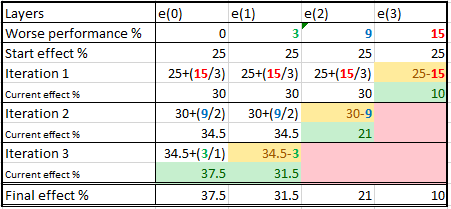
\includegraphics[width=0.5\textwidth]{figures/fredsplit/aggresiveAlgo.png}
    \centering
    \caption{Example of aggressive splitting of layer effect based on performance}
    \label{fig:fredsplitAgg}
\end{figure}
\begin{figure}
    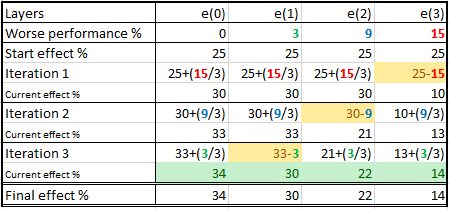
\includegraphics[width=0.5\textwidth]{figures/fredsplit/balancedAlgo.png}
    \centering
    \caption{Example of balanced splitting of layer effect based on performance}
    \label{fig:fredsplitBal}
\end{figure}
